%\chapter{Structure de découpage du projet}
%\section{Structure de découpage du projet}

%Structure de découpage du projet, ou Work Breakdown Structure (WBS) en anglais, est un diagramme hiérarchique, axée sur les tâches et activités que l’équipe de projet doit exécuter pour atteindre les objectifs du projet.

%Dans cette partie nous allons analyser nos tâches. Elles sont divisés en deux parties: Serveur et Arduino. La partie serveur comprend tout ce qui est lié au développement du site ainsi que les scripts qui contrôlent les logiciels, les backups et l'obtention de données. La partie arduino comprend tous les capteurs et modules, l'énergie et les scripts de contrôle des capteurs et manipulation des données.  


%\begin{figure}[h!]
%\centering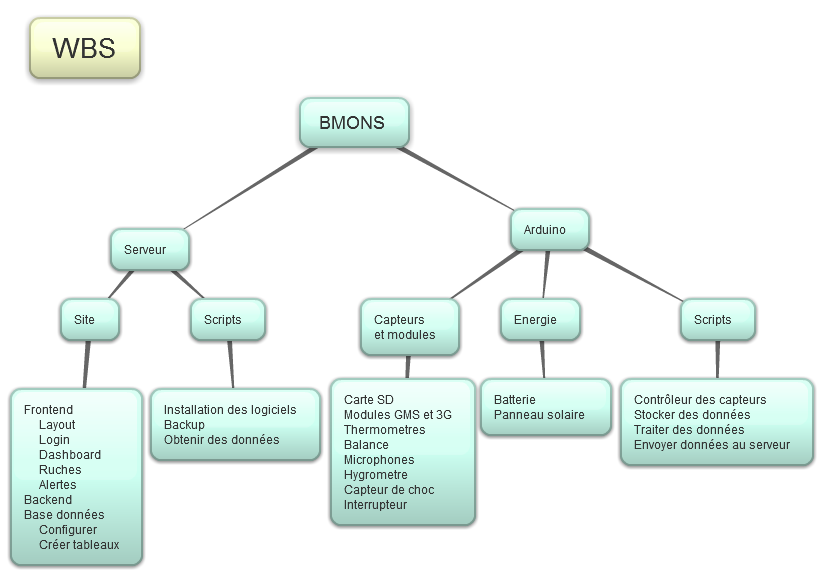
\includegraphics[scale=0.55]{WBS.png}
%\caption{\label{fig:SDP} Structure de découpage du projet du système BMONS}
%\end{figure}

%\clearpage